\documentclass{article}
\usepackage{amsmath}      % Mathematics
\usepackage{amssymb}      % Mathematics
\usepackage{listings}     % Listings
%\usepackage{esint}       % Mathematics (Causing problems with mdframed)
\usepackage{color}        % Listings
\usepackage{courier}      % Listings
\usepackage[oldvoltagedirection]{circuitikz}   % Circuits
\usepackage{titlesec}     % Section Formatting
\usepackage{stmaryrd}     % \mapsfrom arrow. 
\usepackage{mathtools}    % \coloneqq
\usepackage{svg}
\usepackage{import}
\usepackage{pdfpages}
\usepackage{transparent}
\usepackage{xcolor}
\usepackage{blindtext}
\usepackage[hidelinks]{hyperref}
\usepackage{tabularx}
\usepackage{mdframed}
\usepackage{pgfplots}
/home/alex/Meta/templates/tex/dtper_article.tex
%%%%%%%%%%%%%%%%%%%%%%%%%%%%%%%%%%% FORMATTING %%%%%%%%%%%%%%%%%%%%%%%%%%%%%%%%%
\author{Tim Gou}
\title{\textbf{Groups, Analysis, and Geometry Seminars}: Harmonic Analysis of $\mathcal{SU}(2)$}
\date{20th August, 2020}
\usepackage{geometry} % Formatting
%%%%%%%%%%%%%%%%%%%%%%%%%%%%%%%%%%%%%%%%%%%%%%%%%%%%%%%%%%%%%%%%%%%%%%%%%%%%%%%%
\begin{document}

\maketitle

\section{Introduction} 

Suppose $f$ is $2\pi$-periodic, complex valued, integrable over $[0, 2\pi)$, then
\begin{equation}
    \widehat{f}(n) = \frac{1}{2\pi} \int^{2\pi}_{0} f(x) e^{-inx} \ dx
\end{equation}
with $n \in \mathbb{Z}$, is the Fourier transform of $f$. Question: What is $e^{inx}$? Why is $n \in \mathbb{Z}$? Answer: $e^{inx}$ is the character of circle group, denoted by $\mathbb{T}$ (i.e. $e^{ix} \in \mathbb{T}$).

A character is a continuous homomorphism from a locally compact Abelian group $G$ to $\mathbb{T}$: $ \chi : G \rightarrow \mathbb{T} $
where
\begin{equation}
    \chi(gh) = \chi(g)\chi(h)
\end{equation}
for $g,h \in G$. Let's work out $\chi : \mathbb{R} \rightarrow \mathbb{T}$ first, where $\mathbb{R}$ is the group $(\mathbb{R}, +)$. Since $\chi(0)=1$ (identity to identity) and $\chi$ is continuous, then $\exists a > 0$ such that
\begin{equation}
    \int^{a}_{0} \chi(y) \ dy.
\end{equation}
Let $\xi = \int^{a}_{0} \chi(y) \ dy$, then 
\begin{equation}
    \chi(x)\xi = \int^{a}_{0} \chi(x+y) \ dy = \int^{a+x}_{x} \chi(t) \ dt
\end{equation} 
so
\begin{equation}
    \chi(x) = \xi^{-1} \int^{a+x}_{x} \chi(t) \ dt
\end{equation}
and
\begin{equation}
    \begin{split}
        \chi'(x) &= \xi^{-1} \left(\chi(a+x) - \chi(x) \right) \\
                 &= \xi^{-1} \chi(x) \left(\chi(a) - 1\right) \\
                 &= c \chi(x).
    \end{split}
\end{equation}
We have an ODE
\begin{equation}
    \chi'(x) = c \chi(x)
\end{equation}
where solving the equation gives us
\begin{equation}
    \chi(x) = e^{cx}.
\end{equation}
Solving it gives us $\chi(x) = e^{cx}$. Since $| \chi | = 1$, then $c=i\lambda$ with $\lambda \in \mathbb{R}$. Thus $\chi(x) = e^{i\lambda x}$ and we have characters of $\mathbb{R}$, all the $\chi_{\lambda}$ form a dual group of $\mathbb{R}$, denoted by $\widehat{\mathbb{R}}$. 

Since we identify each $\chi_{\lambda}$ with $\lambda \in \mathbb{R}$, then 
\begin{equation}
    \widehat{\mathbb{R}} \cong \mathbb{R}.
\end{equation}

To work out $\widehat{\mathbb{T}}$, notice that 
\begin{equation}
    \mathbb{T} \cong \mathbb{R} / 2\pi \mathbb{Z}
\end{equation}
i.e. each element in $[0, 2\pi)$ is a representative of the cosets of $\mathbb{R} / 2 \pi \mathbb{Z}$. Suppose $x, y \in \mathbb{R}/2\pi \mathbb{Z}$ and $x+y = 2\pi$, then
\begin{equation}
    \chi(x+y) = \chi(0) = 1 = e^{i\lambda (x+y)}
\end{equation}
we know $\lambda \in \mathbb{R}$, but the only way $e^{i\lambda(x+y)}=1$ is that $\lambda \in \mathbb{Z}$. So all the $\chi_{n}(x) = e^{inx}$ for the dual group $\widehat{\mathbb{T}}$, and 
\begin{equation}
    \widehat{\mathbb{T}} \cong \mathbb{Z}.
\end{equation}
Similarly, we have $\mathbb{R}^{n} \cong \mathbb{R}^{n}$ and $\widehat{\mathbb{T}} \cong \mathbb{Z}^{n}$.

\begin{theorem}
    If $G$ is compact, $\widehat{G}$ is discrete.
\end{theorem} 

In addition, $\{ e^{inx} : n \in \mathbb{Z} \}$ form an orthonormal basis for the Hilbert space $L^{2}(\mathbb{T})$, with respect to its inner product, i.e.
\begin{equation}
    \begin{split}
        \langle e^{imx}, e^{inx} \rangle 
        &= \frac{1}{2\pi} \int^{2\pi}_{0} e^{imx} e^{-inx} \ dx \\
        &= \delta_{mn} = 
        \begin{cases}
            \case 1, \ m=n \\
            \case 0, \ m\neq n \\
        \end{cases}
    \end{split}
\end{equation}

If $G$ is non-Abelian, the analogy generalising the characters is called the \textit{irreducible unitary representation} of $G$:
\begin{equation}
    \sigma : G \rightarrow U(\mathcal{H})
\end{equation}
for $\mathcal{H}$, some Hilbert space. 
\begin{equation}
    \begin{split}
        \sigma(gh) &= \sigma(g)\sigma(h) \\
        \sigma(e) &= \sigma(g g^{-1}) = \sigma(g)\sigma(g^{-1}) = \sigma(g)\sigma(g)^{*} \\
        \langle \sigma(g)u, \sigma(g)v \rangle &= \langle u,v \rangle \\
    \end{split}
\end{equation}
for $u,v \in \mathcal{H}$. We'll look at the irreducible representations of $\mathcal{SU}(2)$. $\mathcal{SU}(2)$ is the first compacy and non-abelian group we normally look at in Harmonic Analysis. 

\section{Aspects of $\mathcal{SU}(2)$} 

We begin by looking at $\mathcal{U}(2)$, a group of unitary transformations of $\mathbb{C}^{2}$. 
\begin{equation}
    A A^{*} = A^{*}A = I, A \in \mathcal{U}(2)
\end{equation}
$\mathcal{SU}(2) \subset \mathcal{U}(2)$ where elements of $\mathcal{SU}(2)$ have determinant 1. 
\begin{equation}
    \begin{cases}
        \case \det\left( AB \right) = \det\left( A \right) \det\left( B \right), \ A,B \in \mathcal{SU}(2) \\
        \case \det\left( I \right) = \det\left( A A^{-1} \right) = \det\left( A \right) \det\left( A^{-1} \right)
    \end{cases}
\end{equation}
suppose 
\begin{equation}
    \begin{pmatrix}
        \alpha & \beta \\
        \gamma & \eta \\
    \end{pmatrix} \in \mathcal{U}(2)
\end{equation}
then, $| \alpha |^{2} + | \beta |^{2} = | \gamma |^{2} + | \eta |^{2} = 1$ and $\alpha \overline{\gamma} + \beta \overline{\eta} = 0$. So,
\begin{equation}
    \begin{pmatrix}
        \alpha \\ \beta \\
    \end{pmatrix},
    \begin{pmatrix}
        \gamma \\ \eta \\
    \end{pmatrix}
\end{equation}
are unit vectors and orthogonal. Thus, 
\begin{equation}
    \begin{pmatrix}
        \gamma \\ \eta \\
    \end{pmatrix}
    = e^{i\theta}
    \begin{pmatrix}
        -\overline{\beta} \\ \overline{\alpha} \\
    \end{pmatrix},
    \ \theta \in \mathbb{R}.
\end{equation}
Hence we have
\begin{equation}
    A =
    \begin{pmatrix}
        \alpha & \beta \\
        -e^{i\theta}\overline{\beta} & e^{i\theta}\overline{\alpha} \\
    \end{pmatrix}
    \ \in \mathcal{U}(2)
\end{equation}
with $\text{det}\left( A \right) = e^{i\theta}$ and $\text{det}\left( A^{*} \right) = e^{-i\theta}$.
If $A \in \mathcal{SU}(2)$, then 
\begin{equation}
    A = 
    \begin{pmatrix}
        \alpha & \beta \\
        -\overline{\beta} & \overline{\alpha}
    \end{pmatrix}
    \in \mathcal{SU}(2).
\end{equation}
\begin{equation}
    \mathcal{SU}(2) = 
    \left\{ 
        \begin{pmatrix}
            \alpha & \beta \\
            -\overline{\beta} & \overline{\alpha}
        \end{pmatrix}
        :
        | \alpha |^{2} + | \beta |^{2} = 1
    \right\}
\end{equation}
where $\alpha, \beta \in \mathbb{C}$. If $\alpha = a+ib$ and $\beta = c+id$ then
\begin{equation}
    \begin{split}
        | \alpha |^{2} + | \beta |^{2} &= 1 \\
        \left| \sqrt{a^{2} + b^{2}} \right|^{2} + \left| \sqrt{c^{2} + d^{2}} \right|^{2} &= 1 \\
        {a^{2} + b^{2}} + {c^{2} + d^{2}} &= 1 \\
    \end{split}
\end{equation}
and so $\mathcal{SU}(2) \cong S^{3}$, the $3-$sphere. $\mathbb{T} \subset \mathcal{SU}(2)$
\begin{equation}
    \mathbb{T} = \left\{ 
        \begin{pmatrix}
            \alpha & 0 \\
            0 & \overline{\alpha}
        \end{pmatrix}
        :
        | \alpha | = 1
    \right\}
\end{equation}

\begin{theorem}
    Given $A \in \mathcal{SU}(2)$, $\exists V \in \mathcal{SU}(2)$, such that 
    \begin{equation}
        V A V^{-1} = T
    \end{equation} 
    for some $T \in \mathbb{T}$.
\end{theorem}

\begin{proof}
    If $A \in \mathcal{U}(2)$, $A$ is normal, then by the \textit{spectral theorem}, $\exists V \in \mathcal{U}(2)$ such that
    \begin{equation}
        VA v^{-1} = 
        \begin{pmatrix}
            \alpha & 0 \\
            0 & \beta \\
        \end{pmatrix}
    \end{equation}
    with $| \alpha | = | \beta | = 1$.
\end{proof}

If $A \in \mathcal{SU}(2)$, then $\beta = \overline{\alpha}$ . So, $V \in \mathcal{U}(2)$ , $A \in \mathcal{SU}(2)$, we have
\[
    VAV^{-1} = 
    \begin{pmatrix}
        \alpha & 0 \\
        0 & \overline{\alpha}
    \end{pmatrix}.
\]
To make $V$ special unitary, let $\tilde{V} = \det\left( V \right)^{1/2}V$ such that $\det\left( \tilde{V} \right) = 1$ and we have $\tilde{V}A\tilde{V}^{-1}=T$.

$\mathcal{SU}(2)$ is a compact, connected, Lie group, (?) we have a theorem to generalise this conjugation relation.

\begin{theorem}
    If $G$ is a compact, connected, Lie group, $\mathbb{T}$ is its maximal torus, then for $\chi \in G$, $\exists g \in G$, such that
    \begin{equation}
        g \chi g^{-1} = t \quad : \quad t \in \mathbb{T}.
    \end{equation}
\end{theorem}

\begin{theorem}
    (proposition?) Define $O_{x} = \{ g \chi g^{-1} : g \in G \}$, then for $\mathcal{SU}(2)$, every $O_{x}$ intersects $\mathbb{T}$ at exactly two points.
\end{theorem}

\begin{proof}
    We have $g \chi g^{-1} = t$ , let
    \[
        g_1 = 
        \begin{pmatrix}
            0 & 1 \\
            -1 & 0 \\
        \end{pmatrix}
        \Rightarrow
        g^{-1} = 
        \begin{pmatrix}
            0 & -1 \\
            1 & 0 \\
        \end{pmatrix}
    \]
    so 
    \[
        \begin{split}
            (g_1 g) \chi (g_1 g)^{-1} &= 
            \begin{pmatrix}
                0 & 1 \\
                -1 & 0 \\
            \end{pmatrix}
            \begin{pmatrix}
                e^{i\theta} & 0 \\
                0 & e^{-i\theta} \\
            \end{pmatrix}
            \begin{pmatrix}
                0 & -1 \\
                1 & 0 \\
            \end{pmatrix} \\
                                      &=
            \begin{pmatrix}
                e^{-i\theta} & 0 \\
                0 & e^{i\theta}
            \end{pmatrix}
        \end{split}
    \]
\end{proof}

Now, we describe the irreducible representations of $\mathcal{SU}(2)$. $\mathcal{SU}(2)$ naturally acts on $\mathbb{C}^{2}$ ($\sigma$ is just the identity mapping) i.e.
\begin{equation}
    \begin{pmatrix}
        \alpha & \beta \\
        -\overline{\beta} & \overline{\alpha} \\
    \end{pmatrix}
    \begin{pmatrix}
        z \\ w
    \end{pmatrix} 
    = 
    \begin{pmatrix}
        \alpha z + \beta w \\
        - \overline{\beta}z + \overline{\alpha}w
    \end{pmatrix}
\end{equation}

We are interested in $\mathcal{SU}(2)$ acting on the vector spaces which are built out of $\mathbb{C}^{2}$, e.g.
\begin{equation}
    L^{2}(\mathcal{SU}(2)) \cong L^{2}(S^{3})
\end{equation}
made up of functions
\begin{equation}
    f : \mathbb{C}^{2} \rightarrow \mathbb{C}
\end{equation}
and let $P$ be the space of all polynomials with two complex variables, i.e. $f \in P$ such that
\begin{equation}
    f(z,w) = \sum_{j,k}^{} a_{jk} z^{j} w^{k}
\end{equation}
and 
\begin{equation}
    P \subset L^{2}(S^{3}) 
\end{equation}
where both spaces are infinite dimensional. But $\mathcal{SU}(2)$ is compact, so $d_{\sigma} < \infty$. This means we want to find subspaces of $P$ which are:
\begin{itemize}
    \item finite dimensional
    \item invariant under the action of $\mathcal{SU}(2)$
\end{itemize}

Thus, we pick $P_m$ , the space of homogeneous polynomials of degree $m$. For $f \in P_m$ 
\begin{equation}
    f(z,w) = \sum_{j=0}^{m} a_j z^{m-j} w^{j}
\end{equation}
and let 
\begin{equation}
    A_{\alpha, \beta} := 
    \begin{pmatrix}
        \alpha & \beta \\
        -\overline{\beta} & \overline{\alpha}
    \end{pmatrix},
\end{equation}
we define the regular representation of $\sigma(A_{\alpha,\beta})$ on $f$:
\begin{equation}
    \begin{split}
        \sigma(A_{\alpha, \beta})f(z,w) &= f(A_{\alpha,\beta}(z,w))\\
                                        &= f(\overline{\alpha} z - \beta w, 
                                             \overline{\beta}z + \alpha w)
    \end{split}
\end{equation}

\begin{theorem}
    $P_m$ is invariant under $\sigma(A_{\alpha,\beta})$.
\end{theorem}

\begin{proof}
    Suppose monomials $z^{m-j}w^{j} \in P_m$ then 
    \begin{equation}
        f(\overline{\alpha}z - \beta w, \overline{\beta}z + \alpha w)
        =
        (\overline{\alpha}z - \beta w)^{m-j} (\overline{\beta}z + \alpha w)^{j} \in P_m.
    \end{equation}
    So, $P_m$ is invariant under $\sigma$.
\end{proof}
Now, we want to define an inner product, i.e.
\begin{equation}
    \langle f,g \rangle = \int_{S^{3}} f \overline{g} \ d\mu
\end{equation}
where $\mu(S^{3})=1$ is the surface measure of $S^{3}$ which is normalised to 1.

So, we'll show monomials $z^{m-j}w^{j}$ are orthogonal in $P$ with respect to this inner product. To achieve this, we use polar coordinates.

Suppose $Z = (z,w) \in C^{2}$ and $Z = r \tilde{z}$, where $\tilde{z} \in S^{3}$, and $r = | z | = \sqrt{| z |^{2} + | w |^{2}}$. We define Lebesgue measure on $\mathbb{C}^{2}$ as 
\begin{equation}
    \begin{split}
        dz &= dz \ dw \\
           &= d_a \ d_b \ d_c \ d_{d} \\
           &= r^{3} \ dr \ d\tilde{\mu}(\tilde{z}) \ : \ \text{(un-normalised)} \\
           &= 2 \pi^{2} r^{3} \ dr \ d\mu (\tilde{z}) \ : \ \text{(normalised)}
    \end{split}.
\end{equation}
To see this, we have $\varphi_1, \varphi_2 \in [0, \pi]$, $\theta \in [0, 2\pi)$. 
\begin{equation}
    \begin{split}
        a &= r \cos\left(\varphi_1\right) \\
        b &= r \sin\left(\varphi_1\right) \sin\left(\varphi_2\right) \\
        c &= r \sin\left(\varphi_1\right) \sin\left(\varphi_2\right) \cos\left(\theta\right) \\
        d &= r \sin\left(\varphi_1\right) \sin\left(\varphi_2\right) \sin\left(\theta\right) .\\
    \end{split}
\end{equation}
The Jacobian matrix is then
\begin{equation}
    J = 
    \begin{bmatrix} 
        \frac{\partial a}{\partial r} & \ldots & * \\
		\vdots & \ddots & \vdots \\
		* & \ldots & \frac{\partial d}{\partial \theta} \\		
    \end{bmatrix}
\end{equation}
giving
\begin{equation}
    \det\left( J \right) = r^{3} \sin^{2}\left(\varphi_1\right) \sin\left(\varphi_2\right).
\end{equation}
The surface measure of $S^{3}$ is exactly
\begin{equation}
    \begin{split}
        \mu(S^{3}) &= \int^{2\pi}_{0} \int^{\pi}_{0} \int^{\pi}_{0}
        \sin^{2}\left(\varphi_1\right) \sin\left(\varphi_2\right)
        d\varphi_1 \ d\varphi_2 \ d\theta
        (?) \\
                   &= 2 \pi^{2}
    \end{split}
\end{equation}

\begin{theorem}
    If $f: \mathbb{C}^{2} \rightarrow \mathbb{C}$  satisfies $f(aZ) = a^{m}f(z)$  for $a>0$ , then
    \begin{equation}
        \int_{S^{3}} f(\tilde{z}) \ d\mu(\tilde{z})
        =
        \frac{1}{\pi^{2} \Gamma(\frac{m+4}{2})} \int_{\mathbb{C}^{2}} f(Z) e^{- | Z |^{2}} \ dZ.
    \end{equation}
\end{theorem}

\begin{proof}
    We integrate in polar coordinates:
    \begin{equation}
        \begin{split}
            \int_{\mathbb{C}^{2}} f(Z) e^{-| Z |^{2}} \ dZ 
            &= 2\pi^{2} \int^{\infty}_{0} \int^{}_{S^{3}} f(r \tilde{z}) e^{-r^{3}} r^{3} \ d\mu(\tilde{z}) \ dr \\
            &= 2\pi^{2} \int^{\infty}_{0} e^{-r^{3}}(?) r^{3} \int^{}_{S^{3}} f(r \tilde{z}) \ d\mu(\tilde{z}) \ dr \\
            &= 2 \pi^{2} \frac{1}{2} \Gamma (\frac{m+4}{2}) \int_{S^{3}} f(\tilde{z}) \ d\mu(\tilde{z})
        \end{split}
    \end{equation}
\end{proof}

\begin{theorem}
    If $p,q,r,s \in \mathbb{Z}$ , then 
    \begin{equation}
        \int_{S^{3}} z^{p} \overline{z}^{q} w^{r} \overline{w}^{s} \ d\mu(z,w)
        =
        \begin{cases}
                \case 0 &\ \text{if } p \neq q \text{ or } r \neq s \\
                \case \frac{p! r!}{(p+r+1)!} &\ \text{if } p=q \text{ and } r=s \\
        \end{cases}
    \end{equation}
\end{theorem}

\begin{proof}
    By Prop ??, 
    \begin{equation}
        \int_{S^{3}} z^{p} \overline{z^{q}} w^{r} \overline{w}^{s} \ d\mu(z,w)
        =
        \frac{1}{\pi^{2} \Gamma(\frac{p+q+r+s+4}{2})} \int_{\mathbb{C}} z^{p} \overline{z^{q}} e^{-| z |^{2}} \ dz \cdot \int_{\mathbb{C}} w^{r} \overline{w}^{s}  \ dw
    \end{equation}
    Let $m=p+q+r+s$. Since $f(z) = 1^{m}f(z)$:
    \begin{equation}
        \begin{split}
            \int_{\mathbb{C}} z^{p} \overline{z^{q}} e^{-| z |^{2}} \ dz 
            &=
            \int^{\infty}_{0} \int^{2\pi}_{0} e^{i(p-q)\theta} r^{p+q+1} e^{-r^{2}} \ d\theta \ dr \\
            &= 
            \int^{\infty}_{0} r^{p+q+1} e^{-r^{2}}  \ dr \cdot \int^{2\pi}_{0} e^{i(p-q)\theta} \ d\theta
        \end{split}
    \end{equation}
    If $p\neq q$, then the integral with respect to $\theta$ is 0, and if $p=q$, then
    \begin{equation}
        \int^{2\pi}_{0} e^{i(p-q)\theta} \ d\theta 
        =
        2\pi \frac{1}{2} \Gamma (\frac{2p+2}{2}) 
        = \pi \Gamma ({p+1}) .
    \end{equation}
    Similarly for 
    \begin{equation}
        \int w^{p} \overline{w}^{q} e^{-| w |^{2}} \ dw
        =
        \begin{cases}
            \case 0 &\text{if } r\neq s \\
            \case \pi r! & \text{if } r=s. \\
        \end{cases}
    \end{equation}
    Also, 
    \begin{equation}
        \Gamma \left(\frac{p+q+r+s+4}{2}\right) = (p+r+1)! 
    \end{equation}
    if $p=q$ and $r=s$.
\end{proof}

\begin{theorem}
    The subspaces $P_m$ are mutually orthogonal in $L^{2}(S^{3})$, and 
    \begin{equation}
        \left\{ \sqrt{\frac{(m+1)!}{(m-j)! j!}} z^{m-j}w^{j} \ : \ 0 \leq j \leq m \right\}.
    \end{equation}
\end{theorem}

\begin{proof}
   By the previous theorem ??. 
\end{proof}

For each $P_m$, we can define the representation $\sigma_m$ acting on it, and we can quickly access the information of $\sigma_m$ by looking at its (trace) characters. Let $A_{\alpha, \sigma} \in \mathbb{T}$, then
\begin{equation}
    \sigma_m(A_{\alpha, 0(?)})(z^{m-j}w^{j}) = e^{i(m-zj)\theta}z^{m-j}w^{j}.
\end{equation}
Therefore, each orthogonal vector $z^{m-j}w^{j}$ of $P_m$ is an eigenvector of $\sigma_m(A_{\alpha, 0(?)})$. This means we can write
\begin{equation}
    \sigma_m(A_{\alpha,0}) =
    \begin{bmatrix} 
        e^{im\theta} & 0  & 0  & 0  & 0  \\
        0 & e^{i(m-2)\theta} &0 &0  &0  \\
        0  &0 & \ddots &0  &0  \\
        0  &0 &0  & e^{-i(m-2)\theta} &0  \\
        0  &0  &0 &0    & e^{-im\theta} \\		
    \end{bmatrix}
\end{equation}
So, 
\begin{equation}
    \begin{split}
        \text{Tr}\left(\sigma_m(A_{\alpha, 0})\right) &=
        \sum_{j=0}^{m} e^{i(m-2j)\theta} \\
        &=\frac{e^{i(m+2)\theta}-e^{-im\theta}}{e^{2i\theta}-1} \\
        &= \frac{e^{i(m+1)\theta}-e^{-i(m+1)\theta}}{e^{i\theta}-e^{-i\theta}}\\
        &= \frac{ \sin\left((m+1)\theta\right)}{ \sin\left(\theta\right)}
    \end{split}
\end{equation}
By theorem ??, every $\chi \in \mathcal{SU}(2)$ can be written as 
\begin{equation}
    \chi = g^{-1}t g \ : \ \exists g \in \mathcal{SU}(2), t \in \mathbb{T}. 
\end{equation}
So, by the cyclic property of trace we have
\begin{equation}
    \begin{split}
        \text{Tr}\left(\sigma_m(g^{-1}t g)\right) &= 
        \text{Tr}\left(\sigma_m(g)^{-1}\sigma_m(t)\sigma_m(g)\right) \\
        &= \text{Tr}\left(\sigma_m(t)\right).
    \end{split}
\end{equation}
Hence, we could conclude that every $\sigma_m$ looks like $\frac{ \sin\left((m+1)\theta\right)}{ \sin\left(\theta\right)}$.

\begin{figure}
\begin{center}
    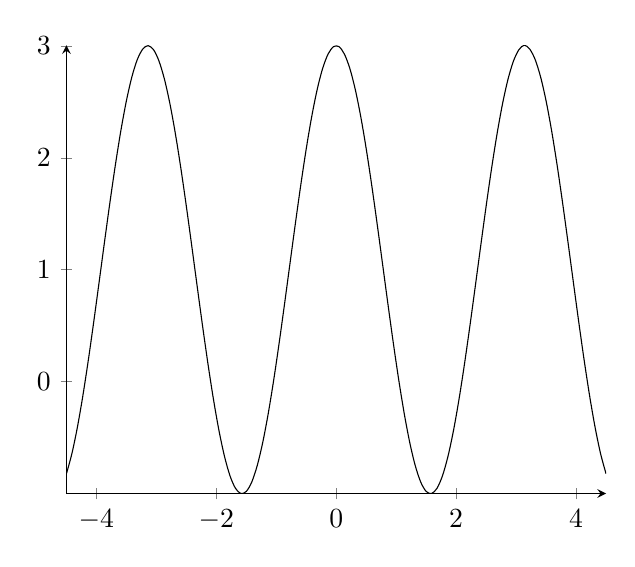
\begin{tikzpicture}
        \begin{axis}[axis lines = left, domain=-4.5:4.5, samples=100, smooth]
            \addplot[smooth] {sin(3*deg(x))/sin(deg(x))}; 
        \end{axis}
    \end{tikzpicture}
    \caption{An example of $\frac{ \sin\left((m+1)\theta\right)}{ \sin\left(\theta\right)}$when $m=2$.}
\end{center}
\end{figure}

The trace character simply does not give enough information about $\sigma_m$, so we still need to work out the matrix coefficients of $\sigma_m$. Suppose 
\begin{equation}
    e_{j}(z,w) = \sqrt{\frac{(m+1)!}{(m-j)!j!}}z^{m-j}w^{j}
\end{equation}
and let 
\begin{equation}
    \sigma_m(\alpha, \beta) = \sigma_m(A_{\alpha,\beta}).
\end{equation}
Then the matrix coefficient $\sigma^{jk}_{m}(\alpha,\beta)$ can be recovered by
\begin{equation}
    \sigma^{jk}_{m}(\alpha,\beta)= \langle \sigma_m(\alpha,\beta)e_k, e_j \rangle
\end{equation}
where the right-hand-side is the inner product on $L^{2}(S^{3})$ . Following this we have
\begin{equation}
    \begin{split}
        \sigma_m(\alpha, \beta)\cdot e_k (z,w) &=
        \sqrt{\frac{(m+1)!}{(m-k)!k!}}(\overline{\alpha}z - \beta w)^{m-k}(\overline{\beta}z+\alpha w)^{k} \\
        &= \sum_{j=0}^{m} \sigma^{jk}_{m}(\alpha,\beta)e_j(z,w) \\
        &= \sum_{j=0}^{m} \sqrt{\frac{(m+1)!}{(m-j)!j!}} \sigma^{jk}_{m}(\alpha,\beta)z^{m-j}w^{j}.
    \end{split}
\end{equation}
Thus, we have
\begin{equation}
        \sum_{j=0}^{m} \sqrt{\frac{(m+1)!}{(m-j)!j!}} \sigma^{jk}_{m}(\alpha,\beta)z^{m-j}w^{j}
        =
        (\overline{\alpha}z - \beta w)^{m-k}(\overline{\beta}z+\alpha w)^{k}. \\
\end{equation}
We can solve this by multiplying out the right hand side and matching the coefficients of $z^{m-j}w^{j}$. However, observe and realise that if we let $z=1$, $w=e^{ix}$, then we have
\begin{equation}
    \sum_{j=0}^{m} \sigma^{jk}_{m}(\alpha,\beta)e^{ij\chi} 
    =
    \underbrace{
    (\overline{\alpha}- \beta e^{i\chi})^{m-k}(\overline{\beta}+\alpha e^{i\chi})^{k}}_{ \in L^{2}(\mathbb{T})(?)}
\end{equation}
Thus, we have
\begin{equation}
    \sigma^{jk}_{m}(\alpha,\beta) = 
    \sqrt{\frac{(m-j)!j!}{(m-k)!k!}}\cdot \frac{1}{2\pi} \int^{2\pi}_{0} (\overline{\alpha}- \beta e^{i\chi})^{m-k}(\overline{\beta}+\alpha e^{i\chi})^{k} e^{-ij\chi} \ d\chi
\end{equation}
Let us write down $\sigma_m$ for a few $m$.

\[ m = 0 \Rightarrow \sigma_0 = \left[\begin{matrix}1\end{matrix}\right] \] 

\[ m = 1 \Rightarrow \sigma_1 = 
\left[\begin{matrix} \alpha^{} &  \beta^{}\\-  \overline{\beta}^{} &  \overline{\alpha}^{}\end{matrix}\right]
\]%

\[%
    m=2 \Rightarrow \sigma_2 = 
    \left[\begin{matrix}\alpha^{2} &  \sqrt{2} \alpha \beta &  \beta^{2}\\- \sqrt{2} \alpha
    \overline{\beta} & \alpha \overline{\alpha} - \beta \overline{\beta} &  \sqrt{2} \beta
    \overline{\alpha}\\\overline{\beta}^{2} & - \sqrt{2} \overline{\alpha} \overline{\beta}
    & \overline{\alpha}^{2}\end{matrix}\right]
\]%

\[%
    m=3 \Rightarrow \sigma_3 =
    \left[\begin{matrix} \alpha^{3} & \sqrt{3} \alpha^{2} \beta^{} & \sqrt{3} \alpha^{}
    \beta^{2} &  \beta^{3}\\- \sqrt{3} \alpha^{2} \overline{\beta}^{} & - 2 \alpha^{} \beta^{}
    \overline{\beta}^{} +  \alpha^{2} \overline{\alpha}^{} & 2 \alpha^{} \beta^{} \overline{\alpha}^{}
    -  \beta^{2} \overline{\beta}^{} & \sqrt{3} \beta^{2} \overline{\alpha}^{}\\\sqrt{3}
    \alpha^{} \overline{\beta}^{2} & - 2 \alpha^{} \overline{\alpha}^{} \overline{\beta}^{}
    +  \beta^{} \overline{\beta}^{2} &  \alpha^{} \overline{\alpha}^{2} - 2 \beta^{} \overline{\alpha}^{}
    \overline{\beta}^{} & \sqrt{3} \beta^{} \overline{\alpha}^{2}\\-  \overline{\beta}^{3}
    & \sqrt{3} \overline{\alpha}^{} \overline{\beta}^{2} & - \sqrt{3} \overline{\alpha}^{2}
    \overline{\beta}^{} &  \overline{\alpha}^{3}\end{matrix}\right].
\]%
Interestingly, every $\sigma_m$ is irreducible. We demonstrate this using the concept of the Lie algebra, whose details are out of the scope of this talk. For now at least, we have:

\begin{theorem}
    $\sigma_m$ is irreducible for each $m\geq 0$.
\end{theorem}
Also, we have
\begin{Theorem}{Dual}
    \begin{equation}
        \widehat{\mathcal{SU}(2)} = \left\{ [\sigma_m] : m \geq 0 \right\}
    \end{equation}
\end{Theorem}
Note that $[\cdot]$ denotes the equivalence class of $\sigma_m$. It turns out that $\sigma_m$ is equivalent to its contragradient $\overline{\sigma_m}$.
\begin{equation}
    {\sigma^{*}_m}^{(g)} = \sigma(g^{-1})^{T} = \overline{\sigma_m(g)}.
\end{equation}
Now, let's examine the Schur orthogonality relation.
\begin{theorem}
    Let $\sigma$ and $\sigma'$ be irreducible representations of $G$, $\mathcal{E}_{\sigma}$ and $\mathcal{E}_{\sigma'}$ are the linear span of the matrix elements of $\sigma$ and $\sigma'$, respectively.
    \begin{enumerate}
        \item If $[\sigma] \neq [\sigma']$, then $\mathcal{E}_{\sigma} \perp \mathcal{E}_{\sigma'}$.
        \item If $\{ e_j \}$ is any orthonormal basis for $\mathcal{H}_{\sigma}$ and $\sigma_{ij} = \langle \sigma e_j, e_i \rangle$, then
            \[
                \left\{ \sqrt{d_{\sigma}}\sigma_{ij} : i,j=1,\ldots, d_{\sigma} \right\}
            \]
            is an orthonormal basis for $\mathcal{E}_{\sigma}$.
    \end{enumerate}
\end{theorem}
\begin{proof}
    See Folland - Abstract Harmonic Analysis pg.139.
\end{proof}
Finally, we come to the major result of representations of compact groups.
\begin{Theorem}{Peter-Weyl Theorem}
    Let $G$  be a compact group, then 
    \begin{equation}
        L^{2}(G) = \bigoplus^{}_{[\sigma]\in \widehat{G}} \mathcal{E}_{\sigma}
    \end{equation}
    and if $\sigma_{ij}=\langle \sigma e_j, e_i \rangle$, then 
    \begin{equation}
        \left\{ \sqrt{d_{\sigma}}\sigma_{ij} : i,j=1,\ldots,d_{\sigma}, [\sigma] \in \widehat{G} \right\}
    \end{equation}
    is an orthonormal basis for $L^{2}(G)$.
\end{Theorem}
According to the Peter-Weyl theorem, if $f \in L^{2}(G)$, then
\begin{equation}
    f = \sum_{}^{[\sigma]\in \widehat{G}} \sum_{i,j=1}^{d_{\sigma}} a^{\sigma}_{ij} \sigma_{ij},
\end{equation}
and
\begin{equation}
    a^{\sigma}_{ij} = d_{\sigma} \int_{G} f(\chi) \overline{\sigma_{ij}(\chi)} \ d\chi.
\end{equation}
The drawback is we have an orthonormal basis for each $\mathcal{H}_{\sigma}$. If $f \in L^{1}(G)$, $[\sigma]\in \widehat{G}$, and $\sigma$ is the representative of class $[\sigma]$, we define the Fourier transform of  $f$  at $\sigma$  to be
\begin{equation}
    \widehat{f}(\sigma) (?) = \int_{G} f(\chi) \sigma(\chi^{-1}) \ d\chi.
\end{equation}
\end{document}

